\documentclass[11pt]{article}
\usepackage[margin=1.0in]{geometry}
\usepackage{verbatim}
\usepackage{caption}
\usepackage{subcaption}
\usepackage{amsmath, amssymb,latexsym}
\usepackage{graphicx}
\usepackage{float}
\usepackage{listings}
\usepackage{color}

\definecolor{mygreen}{RGB}{28,172,0} % color values Red, Green, Blue
\definecolor{mylilas}{RGB}{170,55,241}

\lstset{language=Matlab,%
    %basicstyle=\color{red},
    basicstyle=\small,
    breaklines=true,%
    morekeywords={matlab2tikz},
    keywordstyle=\color{blue},%
    morekeywords=[2]{1}, keywordstyle=[2]{\color{black}},
    identifierstyle=\color{black},%
    stringstyle=\color{mylilas},
    commentstyle=\color{mygreen},%
    showstringspaces=false,%without this there will be a symbol in the places where there is a space
    numbers=left,%
    numberstyle={\tiny \color{black}},% size of the numbers
    numbersep=9pt, % this defines how far the numbers are from the text
    emph=[1]{for,end,break},emphstyle=[1]\color{red}, %some words to emphasise
    %emph=[2]{word1,word2}, emphstyle=[2]{style},    
}

%\usepackage[pdftex]{graphicx}

\begin{document} 
\begin{titlepage}
	\centering
	{\scshape\LARGE ECEN 5458 \par}
	\vspace{0.5cm}
	{\scshape\Large Sampled Data and Digital Control Systems\par}
	\vspace{2cm}
	{\huge\bfseries Design of Tape Drive Control System\par}
	{\large April 21, 2016\par}
	\vspace{2cm}
	{\Large Zachary \textsc{Vogel} \\
	Partner: Kaitlyn \textsc{Garifi}\par}
	\vfill
	{\large Supervised by\par
	Dr.~Lucy \textsc{Pao}}
	\vfill
\end{titlepage}

\tableofcontents
\newpage


\section{Introduction}

Archival information is mainly stored on modern linear tape drives due to their reliability in data storage (and reading back the data) and their cost effectiveness. However, one of their main limitations is storage density \cite{thesis}. In tape systems, storage density is measured in tracks per inch (TPI) on the tape. Increasing TPI on the tape is one way to improve the storage density of tape systems; however, there are mechanical constraints that make this a challenging problem \cite{thesis}. The constraint that this project will focus on understanding is the servomechanisms of the tape transport system. For this project, we will be focusing on the transfer function from voice coil motor($U(s)$) to servo head position ($Y(s)$). This is given by the following fourth order transfer function \cite{thesis}:
\begin{equation} G(s)= \cfrac{Y(s)}{U(s)}= \cfrac{g\omega_{1}^{2}\omega_{2}^{2}}{(s^2+2\zeta_{1}\omega_{1}s+\omega_{1}^{2})(s^2+2\zeta_{2}\omega_{2}s+\omega_{2}^{2})} \end{equation}
The values of the parameters are: $g=2000$, $\omega_{1}=200\pi$, $\omega_{2}=2000\pi$, $\zeta_{1}=0.0796$, and $\zeta_{2}=0.05$.

\begin{figure}[H]
    \centering
    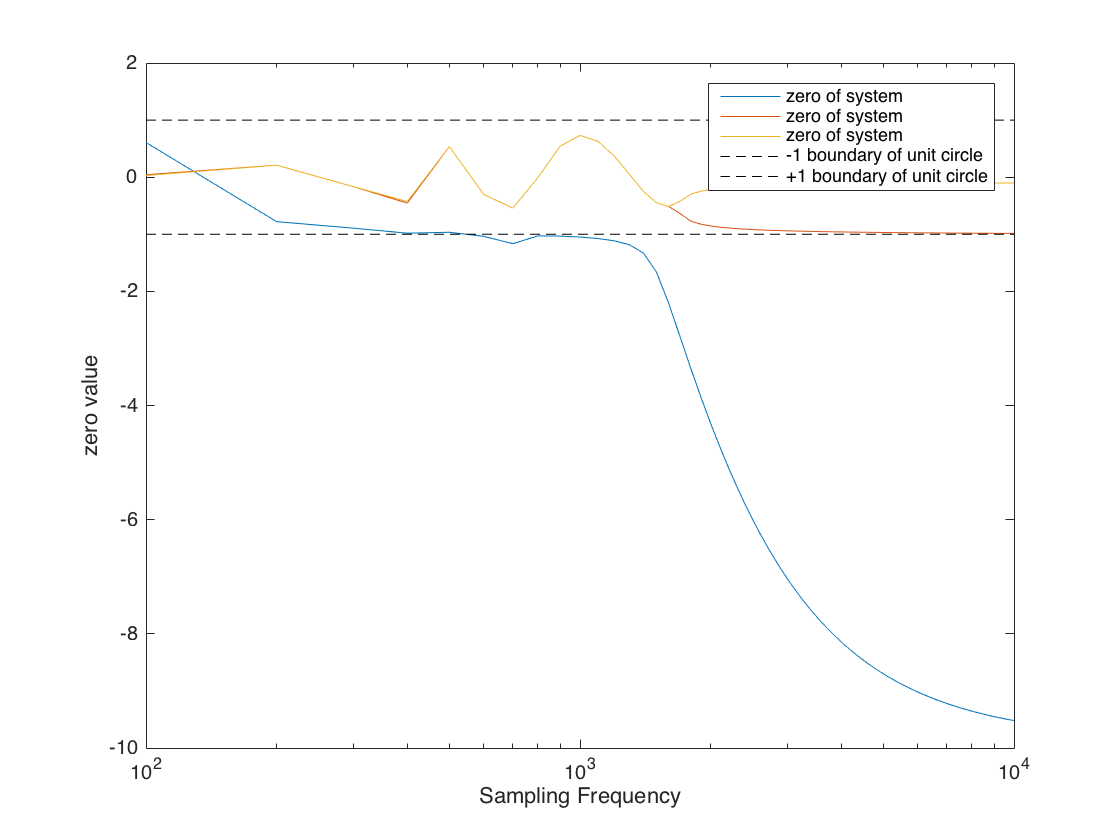
\includegraphics[width=0.7\textwidth]{ECEN5458_SFfig.png}
    \caption{This figure illustrates the pole locations of the discrete-time system using a Zero Order Hold as a function of sampling frequency. As the sampling increases, the system has one non-minimum phase zero. The system was sampled at $10,000$Hz; therefore, the system will have one non-minimum phase zero.} 
    \label{fig:z_vs_SF}
\end{figure}
Next, in order to convert the plant to the discrete-time domain, the sampling frequency for the system was determined. In order to replicate the behavior of a tape drive system, the sampling frequency must be fast due to the desired speed to read/write data at the servo head position. The sampling frequency was chosen to be $10,000$Hz.\\
However, at this frequency, there is a non-minimum phase zero, as illustrated in Figure \ref{fig:z_vs_SF}. As the sampling frequency increases, the system has one non-minimum phase zero. At $10,000$Hz and using the Zero Order Hold method, the discrete-time system is given by the following:

\begin{equation}
    G(z) = \frac{0.1263z^{3}+1.34z^{2}+1.32z+0.1209}{z^{4}+3.555z^{3}+5.045z^{2}-3.418z+0.9298}
\end{equation}
The Bode plot of $G(z)$ is shown in Figure \ref{fig:GzBode}.

\begin{figure}[H]
    \centering
    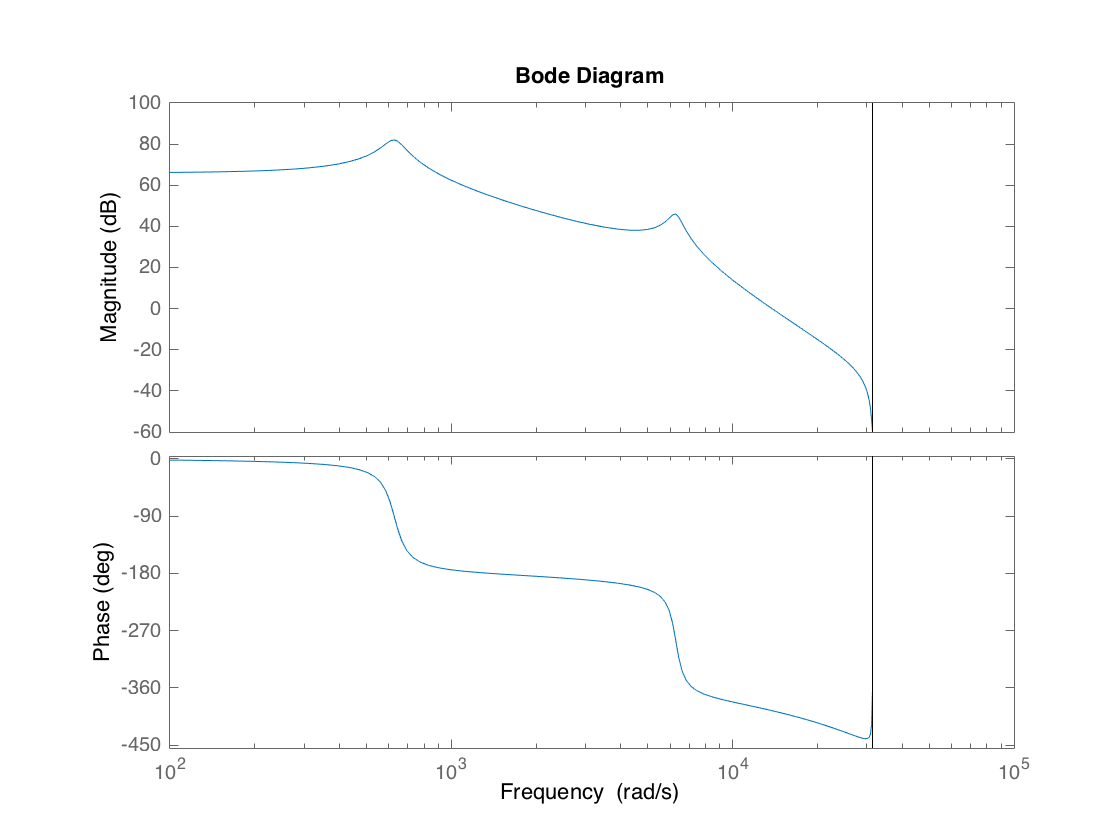
\includegraphics[width=0.67\textwidth]{ECEN5458_project_BODE.png}
    \caption{The Bode plot shows the frequency response of $G(z)$. The two peaks correspond to the resonant frequencies of the system at $200\pi$ and $2000\pi$.} 
    \label{fig:GzBode}
\end{figure}

\begin{figure}[H]
    \centering
    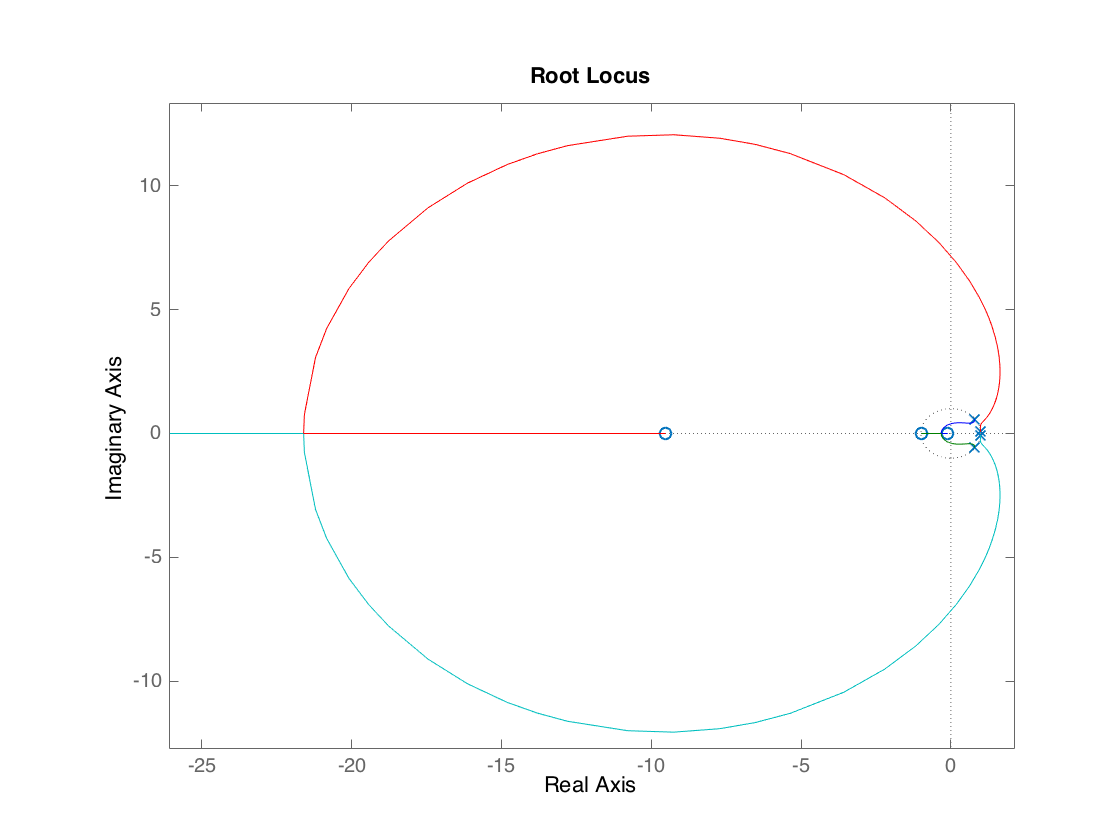
\includegraphics[width=0.67\textwidth]{ECEN5458_gzRL.png}
    \caption{The root locus of the system shows the zero and pole locations as a function of the system gain. The non-minimum phase zero is not shown.} 
    \label{fig:GzRL}
\end{figure}

The root locus of the system, shown in Figure \ref{fig:GzRL}, was also plotted. From the root locus, we can see that the system is only stable for a low gain of about $0.005$ corresponding to $g=2000$. At a gain greater than $0.005$, the poles of the system enter the right half plane. Using the low gain determined above, the zero-pole locations of $0.005\cdot G(z)$ is shown in Figure \ref{fig:gzg_zp}. The step response of the open-loop system $G(z)$ with a gain of $0.005$ is shown in Figure \ref{fig:GzSR}. The step response parameters are shown in Table \ref{tab:gzSR}.

\begin{figure}[H]
    \centering
    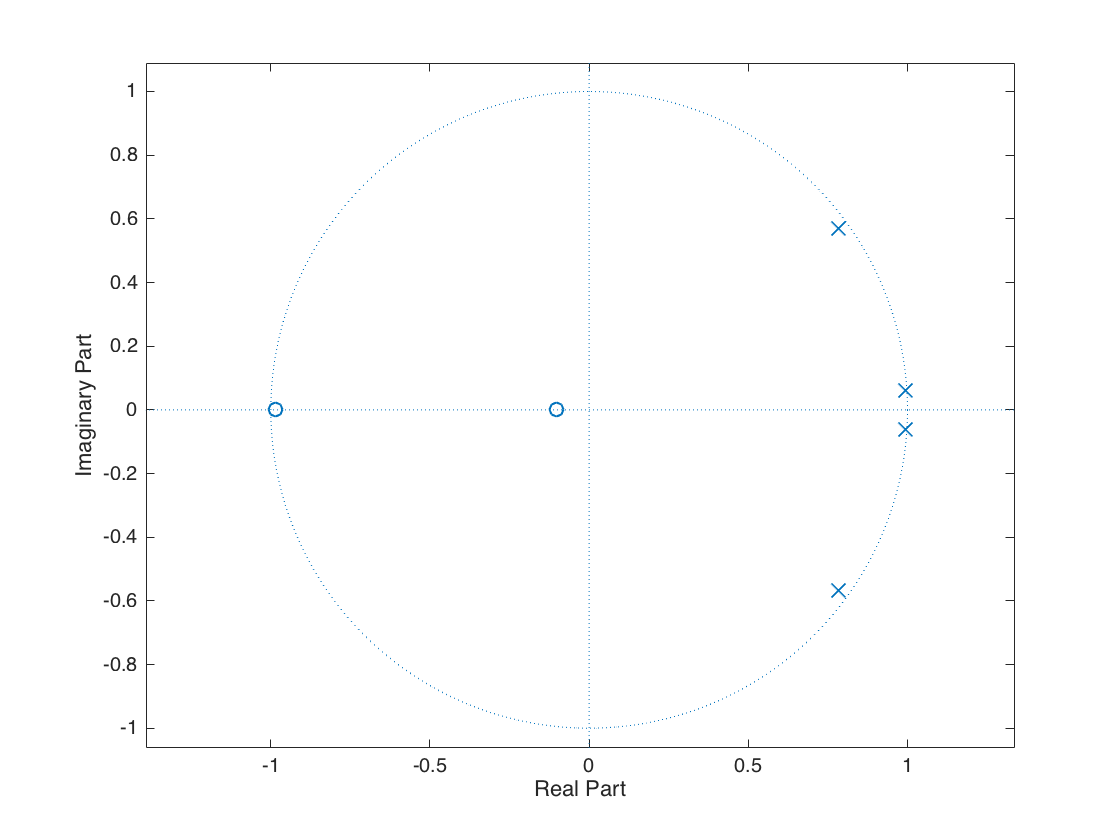
\includegraphics[width=0.7\textwidth]{ECEN5458_gzg_zp.png}
    \caption{The zero and pole locations of $0.005\cdot G(z)$ are shown. (The non-minimum phase zero is not shown.) With this gain, the zeros and poles are located inside the unit circle.} 
    \label{fig:gzg_zp}
\end{figure}

\begin{table}[H]
    \centering
    \begin{tabular}{c|c|c} 
        \hline
        Rise Time & $t_{r}$ & $0.0017$ seconds\\
        Settling Time & $t_{s}$ & $0.0762$ seconds\\
        Overshoot & $M_{p}$ & $78.7895$\\
        \hline
    \end{tabular}
    \caption{Parameters of the Step Response of $0.005 \cdot G(z)$}
    \label{tab:gzSR}
\end{table}

\begin{figure}[H]
    \centering
    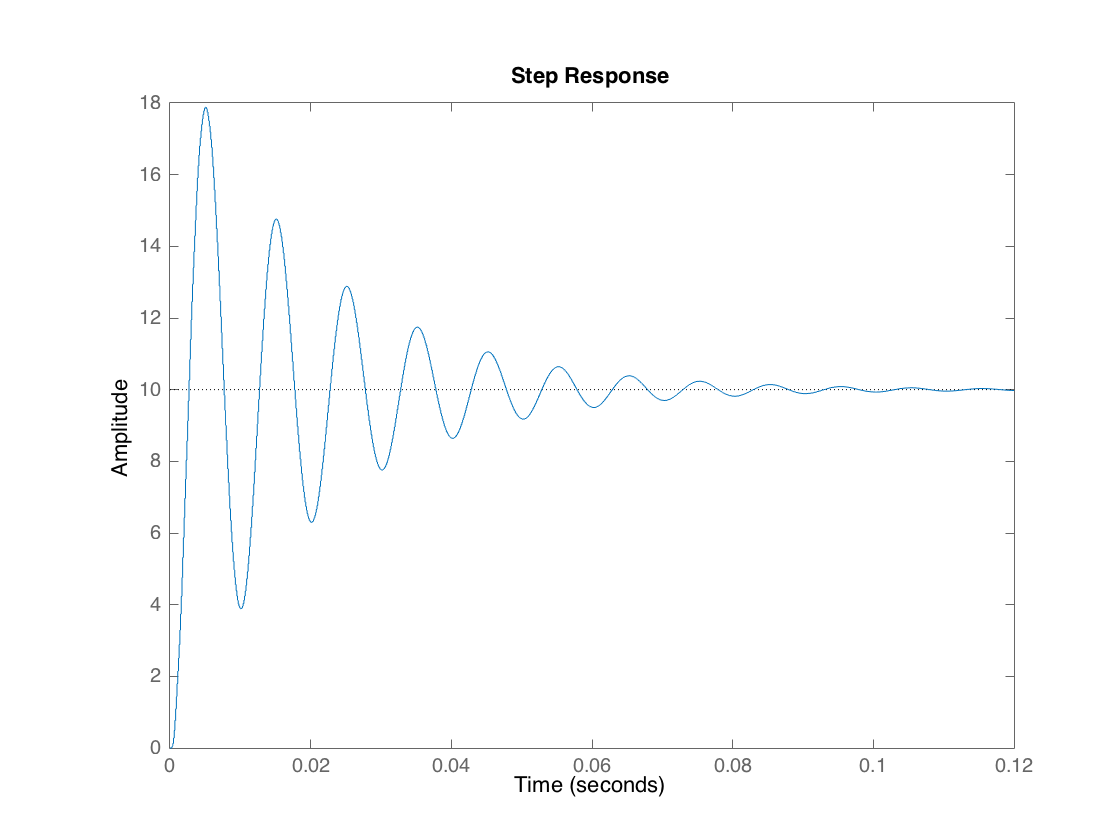
\includegraphics[width=0.7\textwidth]{ECEN5458_gzSR.png}
    \caption{The open-loop step response of $0.005*G(z)$. The parameters of the step response are given in Table \ref{tab:gzSR}. This step response will be used to determine desirable characteristics of the compensated system.}
    \label{fig:GzSR}
\end{figure}



%%%%%%%%%%%%%%%%%%%%%%%%%%%%%%%%%%%%%%%%%%%%%%%%%%%%%%%%%

\section{Analysis}
\subsection{Design using Frequency Domain Tools}
As mentioned in Section 1, the frequency response illustrated by the Bode plot shows that there are two peaks: one at each of the resonant frequencies of the of system. To address the high natural frequencies present in this model at $200\pi$ and $2000\pi$, a notch filter was built for each frequency using the design techniques in \cite{notchF}. From Figure \ref{fig:gzg_zp}, we know that we want to create a notch filter to interact with the poles dominating the response at the natural resonance of the system. The discrete-time domain poles contributing to the $200\pi$ resonant frequency are are $z = 0.9931 \pm 0.0623j$, and the discrete time domain poles contributing to the $2000\pi$ resonant frequency are are $z = 0.7844 \pm 0.5690j$. Thus, the notch filter for each resonant frequency should interact closely with the corresponding poles. \\

Next, a PID controller was designed to improve the response time of the closed-loop system. From the closed-loop system characteristics determined from the step response of the plant in series with the notch filters, the PID controller will be used to reduce the settling time by one order of magnitude to $t_{s} \approx 0.01$. In the tape drive system, this translates to the read/write servo head being positioned on the correct track quickly. To achieve this, a PID controller was built in MATLAB. This was done using the PID Tuner toolbox. The input to this toolbox is the plant and the two notch filters, and the parameters were adjusted until the desired rise time was met. However, a PI controller was basically designed since the derivative term was on the order of $10^{-10}$. The PID controller that achieved this is the following:
\[ D_{PID}(z) = 4.15\times10^{-5} + 0.053\frac{(10^{-4})}{z-1}  \]
The compensator for this system is $D(z) = D_{PID}(z) \cdot N_{200\pi}(z) \cdot N_{2000\pi}$. This is shown in Figure \ref{fig:dzComp}.
\begin{figure}[H]
    \centering
    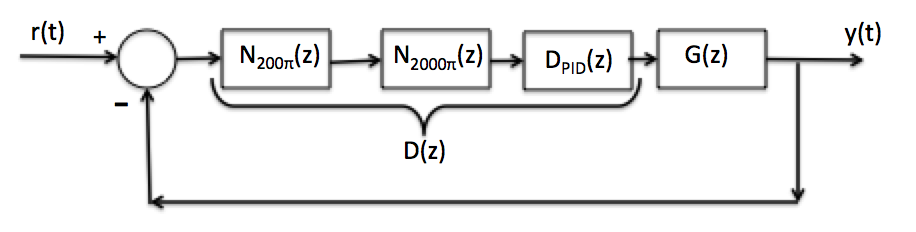
\includegraphics[width=0.7\textwidth]{DzComp.png}
    \caption{Block diagram of the compensator $D(z)$ and plant $G(z)$.}
    \label{fig:dzComp}
\end{figure}

\subsection{Design of Feed-forward Controller}
A feed-forward controller was designed to reject disturbances. The feed-forward controller allows the system to react before the disturbance reaches the output $y(t)$. The block diagram of the feed-forward controller is shown in Figure \ref{fig:d2}. Referring to Figure \ref{fig:d2}, the design of the feed-forward controller will include determining $F(z)$ and $E(z)$. The compensator $D(z)$ used for this design included the PID controller and the two notch filters. Thus, $D(z) = D_{PID}(z)\cdot N_{200\pi}(z) \cdot N_{2000\pi}(z)$. The plant $G(z)$ is our 4th order discrete-time system. In order to design the feed-forward controller, the transfer function from the disturbance $d(t)$ to the output $y(t)$ was determined. The following transfer function was derived assuming a zero reference input.
\[ \frac{Y(z)}{D(z)} = \frac{E(z) + G(z)F(z)}{1+G(z)D(z)} \]

\begin{figure}[H]
    \centering
    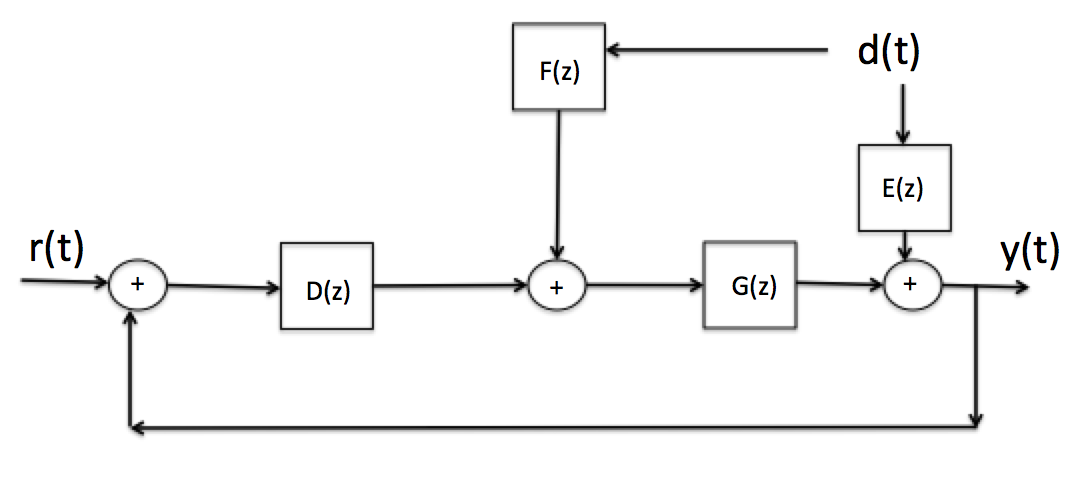
\includegraphics[width=0.7\textwidth]{Diagram2.png}
    \caption{Block diagram of feed-forward controller integrated into unity-feedback block diagram of our system. The block $F(z)$ is the feed-forward controller, which will be designed along with $E(z)$.}
    \label{fig:d2}
\end{figure} 
Here we can assume $E(z)$ is 1. This leads to $F(z)$ needing to be $-G(z)^{-1}$ for the disturbance to get fully rejected. Unfortunately, $G(z)$ has an unstable (non-minimum phase) zero at $-9.5227$ which would lead to an unstable pole if we simply tried flipping the function. Thus, we need to find a good approximation to this inverse. $G(z)$ can be written:
\[G(z)=\cfrac{a_s(z)a_u(z)}{b(z)}\]

where $a_s(z)$ is the stable zeros of the system, $b(z)$ is the poles of the system and $a_u(z)$ is the unstable zeros of the system. This allows us to write $F(z)$ as:
\[F(z)=\cfrac{b(z)a_u(z)^{-1}}{z^la_s(z)}\]

where $l$ is the relative degree of $G(z) + 2$.
The extra poles at zero are to make the system causal. From here we need to find a $a_u(z)^{-1}$ such that $a_u(z)^{-1}*a_u(z)\approx 1$. At this point one has two choices, we can either find $a_u(z)^{-1}$ and try to match the magnitude really well, but suffer non-matching phase at high frequencies or do the opposite and match phase but sacrifice magnitude accuracy. Here we chose to match the magnitude by equating:
\[a_u(z)^{-1}=\cfrac{1+z_o*z}{(1+z_0)^2}\]

With that done, we want the bode plot of $F(z)$ to be compared with that of $G(z)$. This can be seen in Figure \ref{fig:FZGZ}. What is important to note is that the magnitudes are very similar and, at least for low frequencies, the system is 180 degrees out of phase. This means our disturbance will have the same magnitude and negative sign of the original disturbance signal.
\begin{figure}[H]
    \centering
    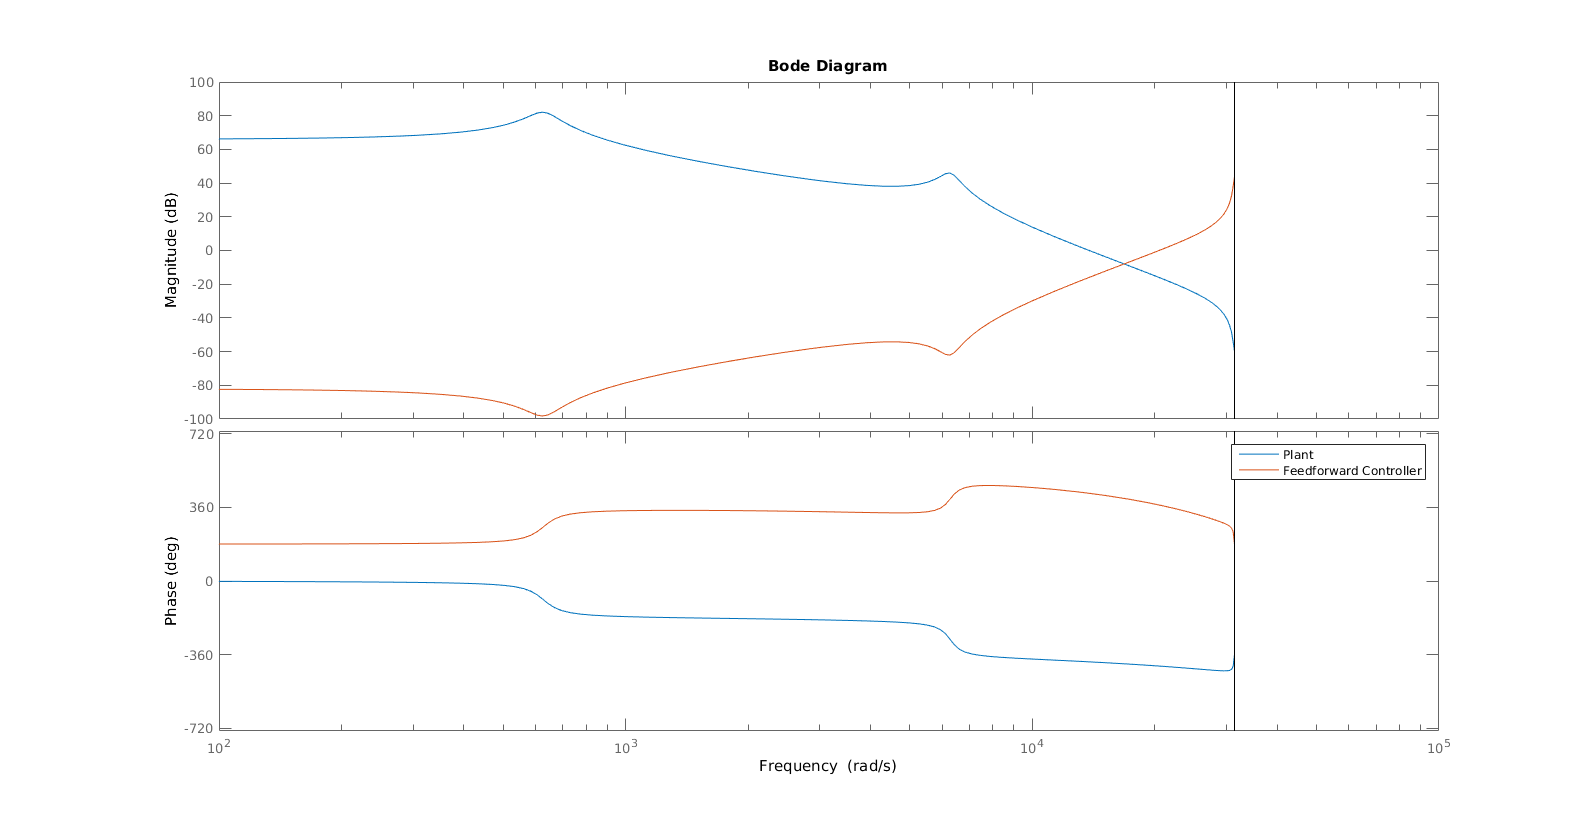
\includegraphics[width=0.9\textwidth]{bode_GZ_Fz.png}
    \caption{The Bode plot of our plant and feedforward controller. Note that the magnitudes are almost inverted and that the phase at the beginning is 180 degrees out of phase.}
    \label{fig:FZGZ}
\end{figure}
\subsection{Design Using State-Space Methods}
This section will describe the design of the state estimator gain matrix, denoted $L$, and the use of state feedback control matrix, denoted $K$, to achieve the desired response. This problem is chiefly concerned with settling time. The open-loop system has a setting time of $0.0762$ seconds as summarized in Table \ref{tab:gzSR}. Our goal for this part of the project, is to use the state-space design methods taught in class to reduce the settling time by one order of magnitude to approximately $t_{s} = 0.007$. 

Given the desired settling time $t_s=0.007$ we knew which region of the unit circle our poles needed to be in to achieve based on the relation:
\[\cfrac{4.6}{t_s}=\zeta\omega_n=\sigma=657.1429\]

Then we can determine the area where our poles need to be by mapping the line at $-\sigma$ in the s plane to the circle defined by $e^{-\sigma*T_{s}}=0.9364$ in the z plane, where $T_{s}=10^{-4}$ is the sampling frequency. Therefore, all of our poles need to be within a circle of radius $0.9364$. We picked the poles $p_{k}$ determined by the state feedback system at $0.5, 0.5\pm 0.5j,$ and $0.8$. We picked the poles $p_{e}$ of the estimator to be faster than the state feedback poles at $0.4, 0.4\pm 0.2j,$ and $0.7$. Then we converted our $G(z)$ to state space and used the Matlab ``place" function to determine the estimator gain matrix $L$ and state feedback gain matrix.
\begin{figure}[H]
    \centering
    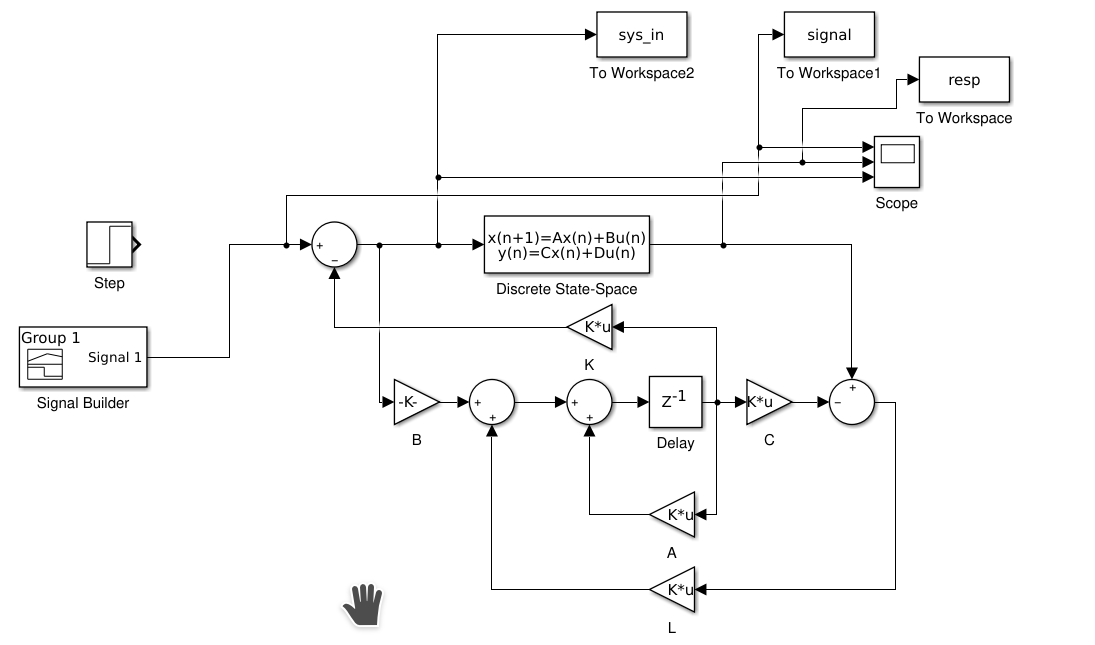
\includegraphics[width=\textwidth]{observer.png}
    \caption{The Simulink Model of our State Observer with State Feedback.}
    \label{fig:observer}
\end{figure}
The state space realization of $G(z)$ is the following:
\[ x(k+1) = \Phi x(k) + \Gamma u(k) \]
\[ y(k) = H x(k) + Ju(k) \]
where \[ \Phi = \left( \begin{array}{cccc}
3.555 & -1.2613 & 0.8546 & -0.4649 \\
4 & 0 & 0 & 0 \\
0 & 1 & 0 & 0\\
0 & 0 & 0.5 & 0 
\end{array} \right)\]
\[\Gamma = \left( \begin{array}{c}
1 \\
 0 \\
 0\\
 0 
\end{array} \right)\]
\[ H = \left( \begin{array}{cccc}
0.1263 & 0.335 & 0.3301 & 0.0605
\end{array} \right)\]
and $J = 0$.
To determine $K$, the input into the ``place" function are the matrices $\Phi$ and $\Gamma$, and the desired state feedback poles $p_{k}$. To determine $L$, the input into the ``place" function are the matrices $\Phi^{T}$ and $H^{T}$, and the desired estimator poles $p_{e}$. We used all of this to make a Simulink model shown in figure \ref{fig:observer}.


%%%%%%%%%%%%%%%%%%%%%%%%%%%%%%%%%%%%%%%%%%%%%%%%%%%%%%%%%%%%%%%%%%%%

\section{Results}
In this section, the results of each of the design sections above will be presented. Section 3.1 presents the results on the design of the two notch filters and the PID controller. Together, the two notch filters and the PID controller make up the compensator $D(z)$. The notch filter designs are evaluated by looking at the pole zero maps of each of the notch filters $N_{200\pi}(z)$ and $N_{2000\pi}(z)$, and seeing which poles of $G(z)$ are affected. The bode plot is also shown to show the affect of the notch filters at the two resonant frequencies of the system. The closed-loop step response is included to show the system response with the addition of the notch filters. Additionally, the closed-loop step response of our system $G(z)$ with compensator $D(z) = D_{PID}(z)\cdot N_{200\pi}(z) \cdot N_{2000\pi}$ is included.\\

Section 3.2 presents the results of the feed-forward controller. Using the $D(z)$ determined above, a feed-forward controller was designed according to the analysis in Section 2.2. To characterize the effectiveness of the feed-forward controller design, a disturbance of varying frequencies were introduced to the system, while the system was reacting to a step input. Simulations are provided for a disturbance of 5 rad/sec, 50rad/sec, and 500rad/sec. \\

Section 3.3 presents the results of designing an additional controller using the state-space methods learned in class. The state feedback matrix $K$ and state estimator matrix $L$ are provided. Then, the step response for the system with the compensator designed in state-space are provided. Additionally, the pole and zero map of the compensator and plant are shown. This will show whether the $K$ and $L$ were able to place the compensator poles were desired. \\



\subsection{Simulation of Notch Filters and PID Controller}
As mentioned in Section 2.1, notch filters were designed to address the natural resonances of the system at $200\pi$Hz and at $2000\pi$Hz. The notch filter for the $200\pi$ frequency is given by the following transfer function:
\begin{equation}
    N_{200\pi}(z) = \frac{z^{2} - 1.996z + 0.9995}{z^{2} - 1.877z + 0.8819}
\end{equation}
The notch filter for the $2000\pi$ frequency is given by the following transfer function:
\begin{equation}
    N_{2000\pi}(z) = \frac{z^{2} - 1.612z + 0.9963}{z^{2} - 0.9397z + 0.1518}
\end{equation}
We put these notch filters in series with the discrete plant $G(z)$ as shown in Figure \ref{fig:NF_BD}. 
\begin{figure}[H]
    \centering
    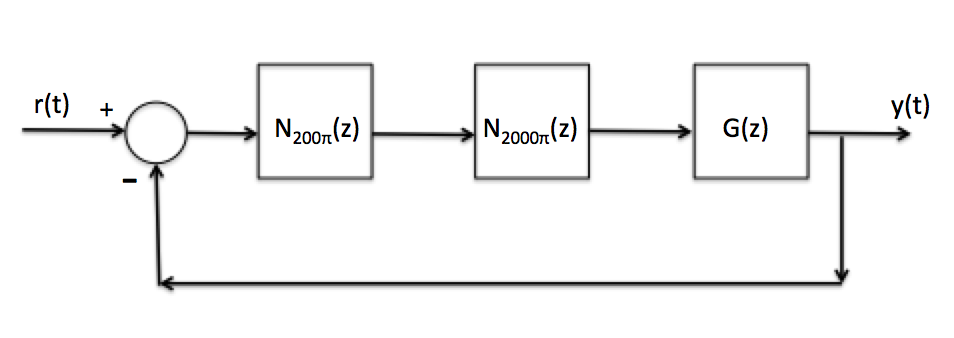
\includegraphics[width=0.7\textwidth]{Diagram1.png}
    \caption{Block diagram of the Notch Filters and Plant $G(z)$ in series.}
    \label{fig:NF_BD}
\end{figure}

To illustrate the effect of the two notch filters on the system, the pole and zero locations are compared. This is shown in Figure \ref{fig:gzNFzp}. The Bode plot of the closed-loop system illustrated in Figure \ref{fig:NF_BD} is shown in Figure \ref{fig:bodeNFGz}. Additionally, the step response of the closed-loop system is shown in Figure \ref{fig:stepNFgz}. From the closed loop step response, the rise time was $0.0007$ seconds, the settling time was $0.0911$ seconds, and the overshoot was $70.85$. Next, the PID controller was added to achieve a settling time of $t_{s} = 0.014$. The step response with the PID controller is also included in Figure \ref{fig:dzStep}.\\


\begin{figure}[H]
    \centering
    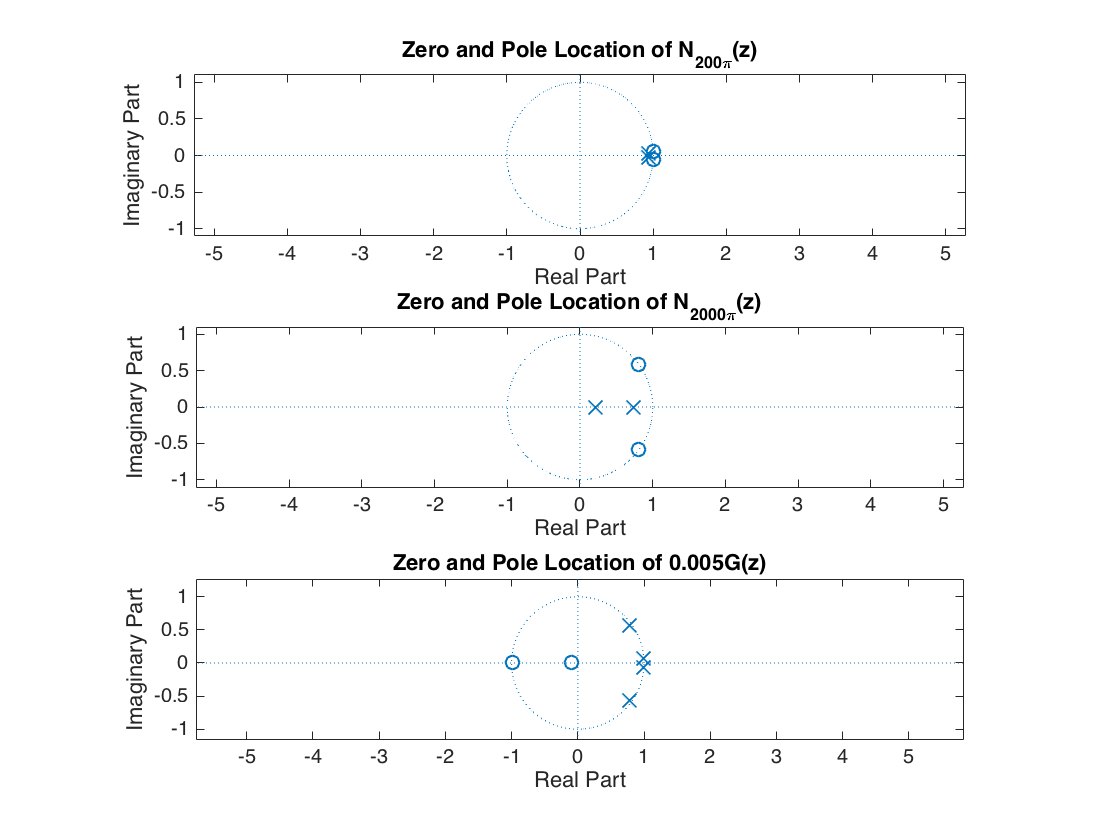
\includegraphics[width=0.7\textwidth]{ECEN5458_gz_NF_zp.png}
    \caption{The pole and zero plots of $N_{200\pi}(z)$ (top), $N_{2000\pi}(z)$ (middle), and $G(z)$ (bottom) are shown to better illustrate the interaction of the poles and zeros of the plant with the poles and zeros of the notch filters.}
    \label{fig:gzNFzp}
\end{figure}  


\begin{figure}[H]
    \centering
    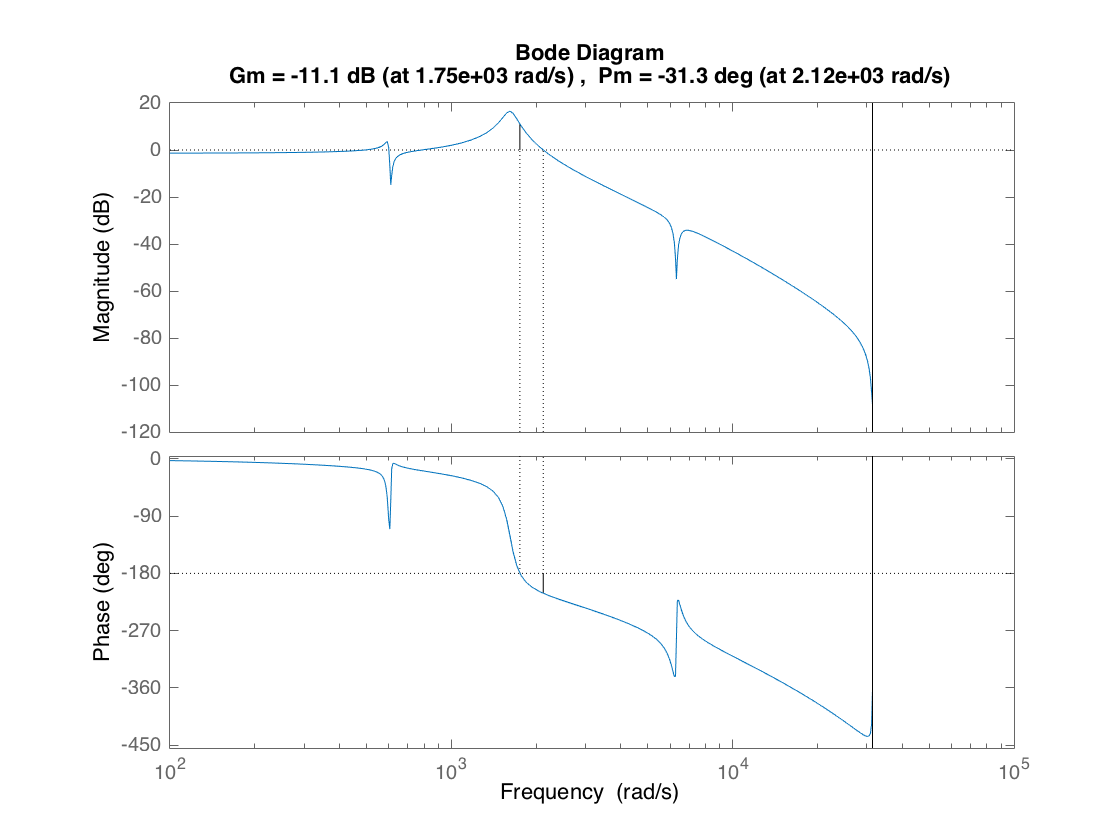
\includegraphics[width=0.7\textwidth]{Bode_NFandGz.png}
    \caption{Bode plot of the closed-loop system of the notch filters, $N_{200\pi}(z)$ and $N_{2000\pi}(z)$, in series with $G(z)$. The Bode plot demonstrates the effect of the notch filters on the frequency response at the two resonant frequencies of the system.}
    \label{fig:bodeNFGz}
\end{figure}  


\begin{figure}[H]
    \centering
    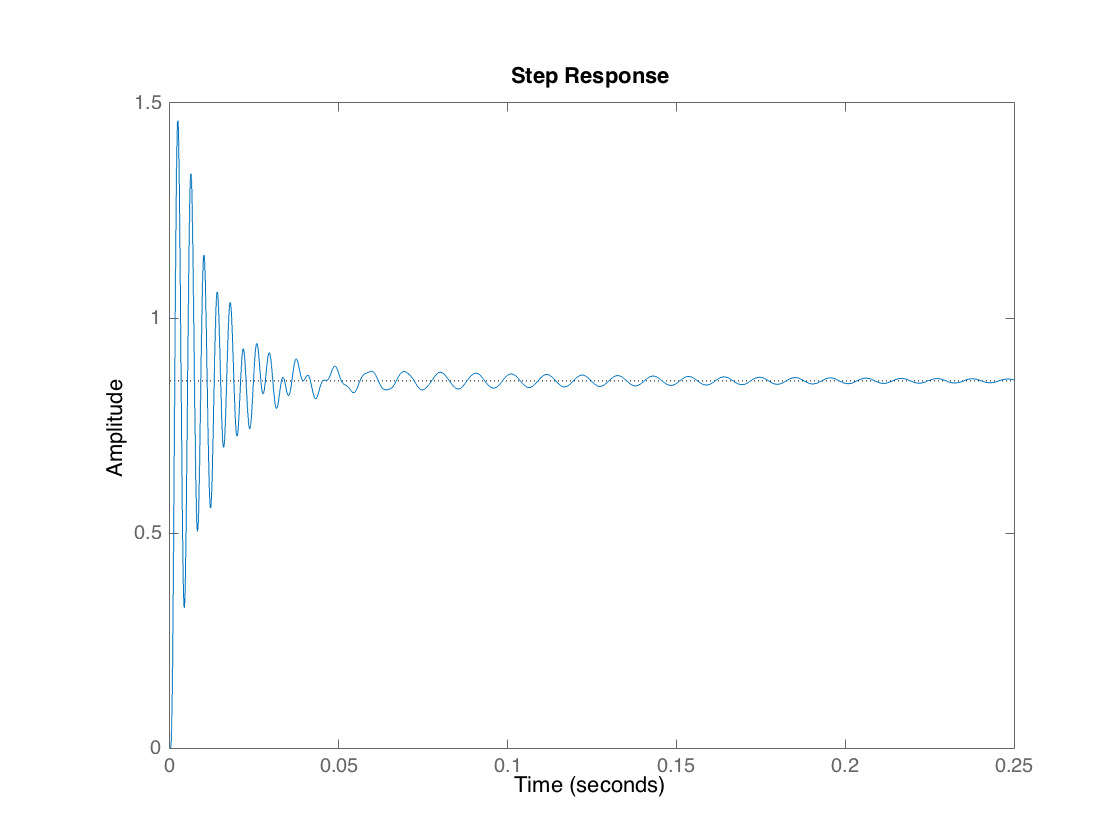
\includegraphics[width=0.7\textwidth]{step_NFandGz.png}
    \caption{The step response of the closed-loop system in Figure \ref{fig:NF_BD} of just the plant and the two notch filters.}
    \label{fig:stepNFgz}
\end{figure}  

\begin{figure}[H]
    \centering
    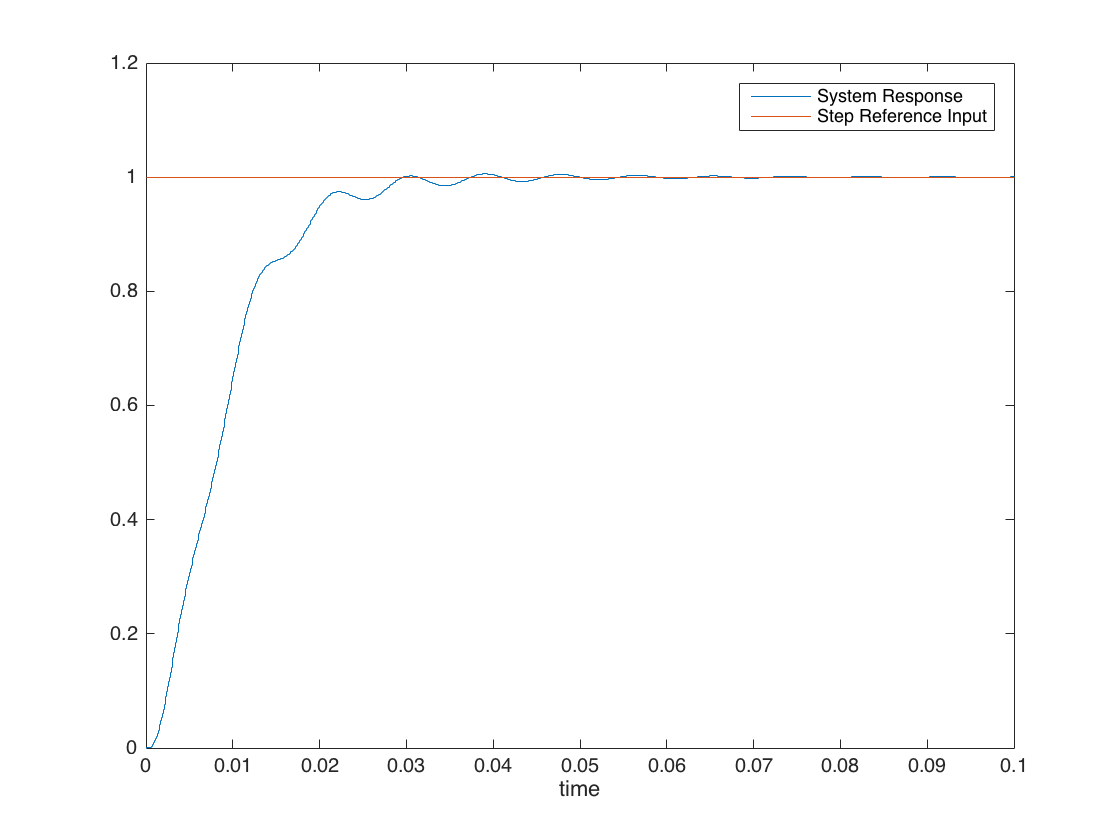
\includegraphics[width=0.7\textwidth]{dzStep.png}
    \caption{Step response of the closed loop system of $G(z)$ and the compensator $D(z)$ which consists of the two notch filters and the PID controller.}
    \label{fig:dzStep}
\end{figure}

\subsection{Simulation of Feed-Forward Controller}
Using the design in Section 2.3, the following feed-forward controller was obtained:
\[ F(z) = \frac{-0.13114(z-0.9853)(z^{2}-1.986z+0.99)(z^{2}-1.569z+0.9391)}{z^{3}(z+0.9853)(z+0.102)} \]
We want to see how the system deals with disturbances at different frequencies while still responding to the step input of 1. The amplitude of the disturbances is always $0.1$. First, we see the response to a $5$ rad/sec wave. At this frequency we get an almost perfect match and can't see any effect from the disturbance. Both the phase and the magnitude are matched really well.

\begin{figure}[H]
    \centering
    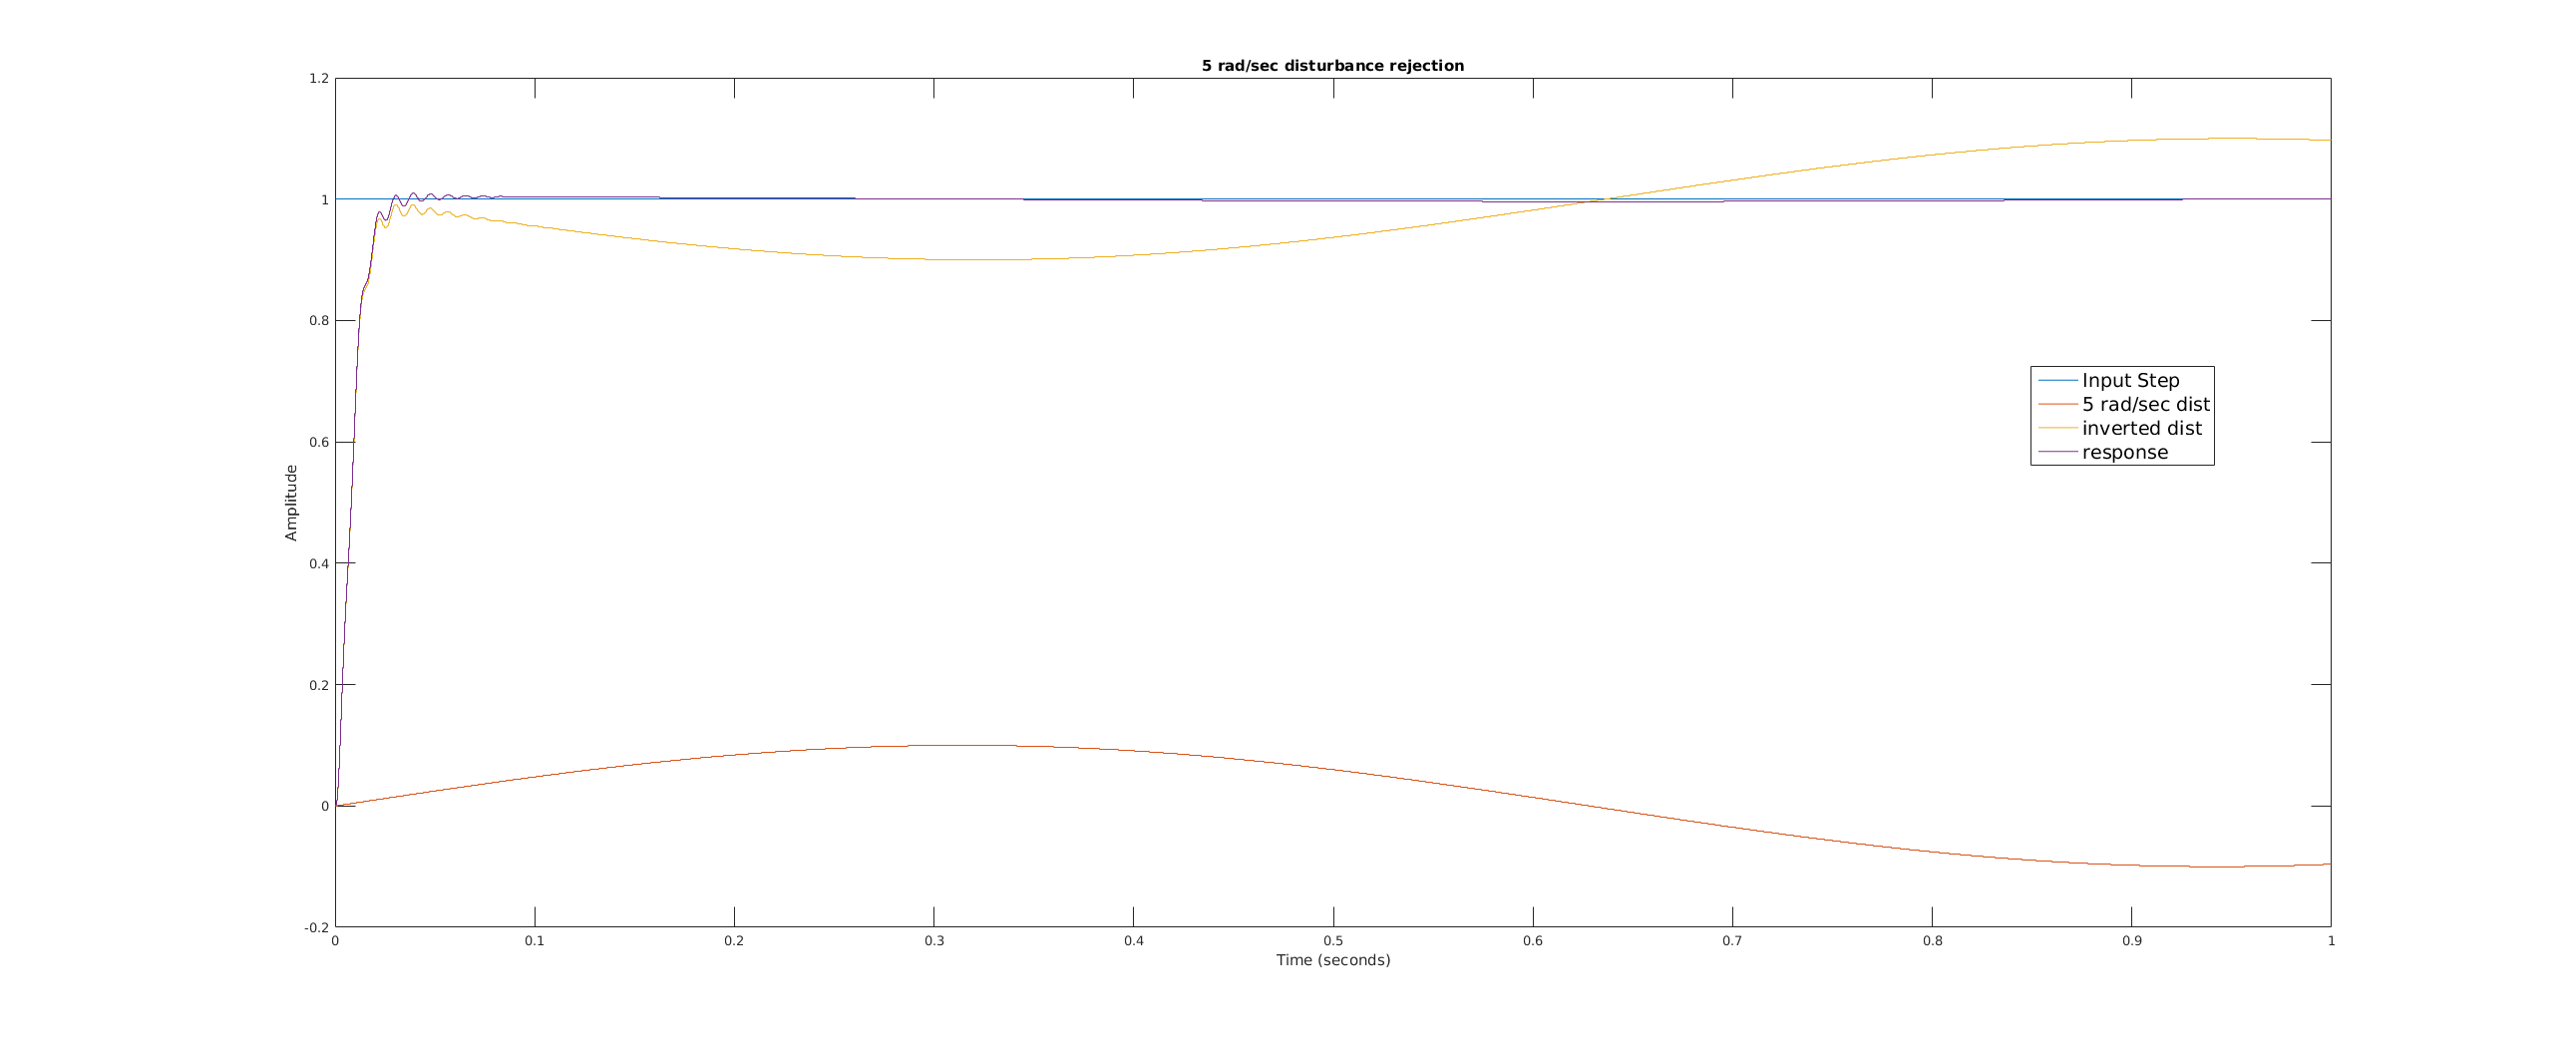
\includegraphics[width=0.9\textwidth]{Dist_5.png}
    \caption{The system response to an amplitude 1 step and a 5 rad/sec disturbance with amplitude 0.1.}
    \label{fig:Dist5radasec}
\end{figure}
Next, at $50$ rad/sec we start to see some oscillatory effects from the disturbance. The feedforward control is struggling at this frequency because the phase is not aligned properly to 180 degrees. In fact, it looks like the disturbance and the inverted disturbance are about 30 degrees out of phase.
\begin{figure}[H]
    \centering
    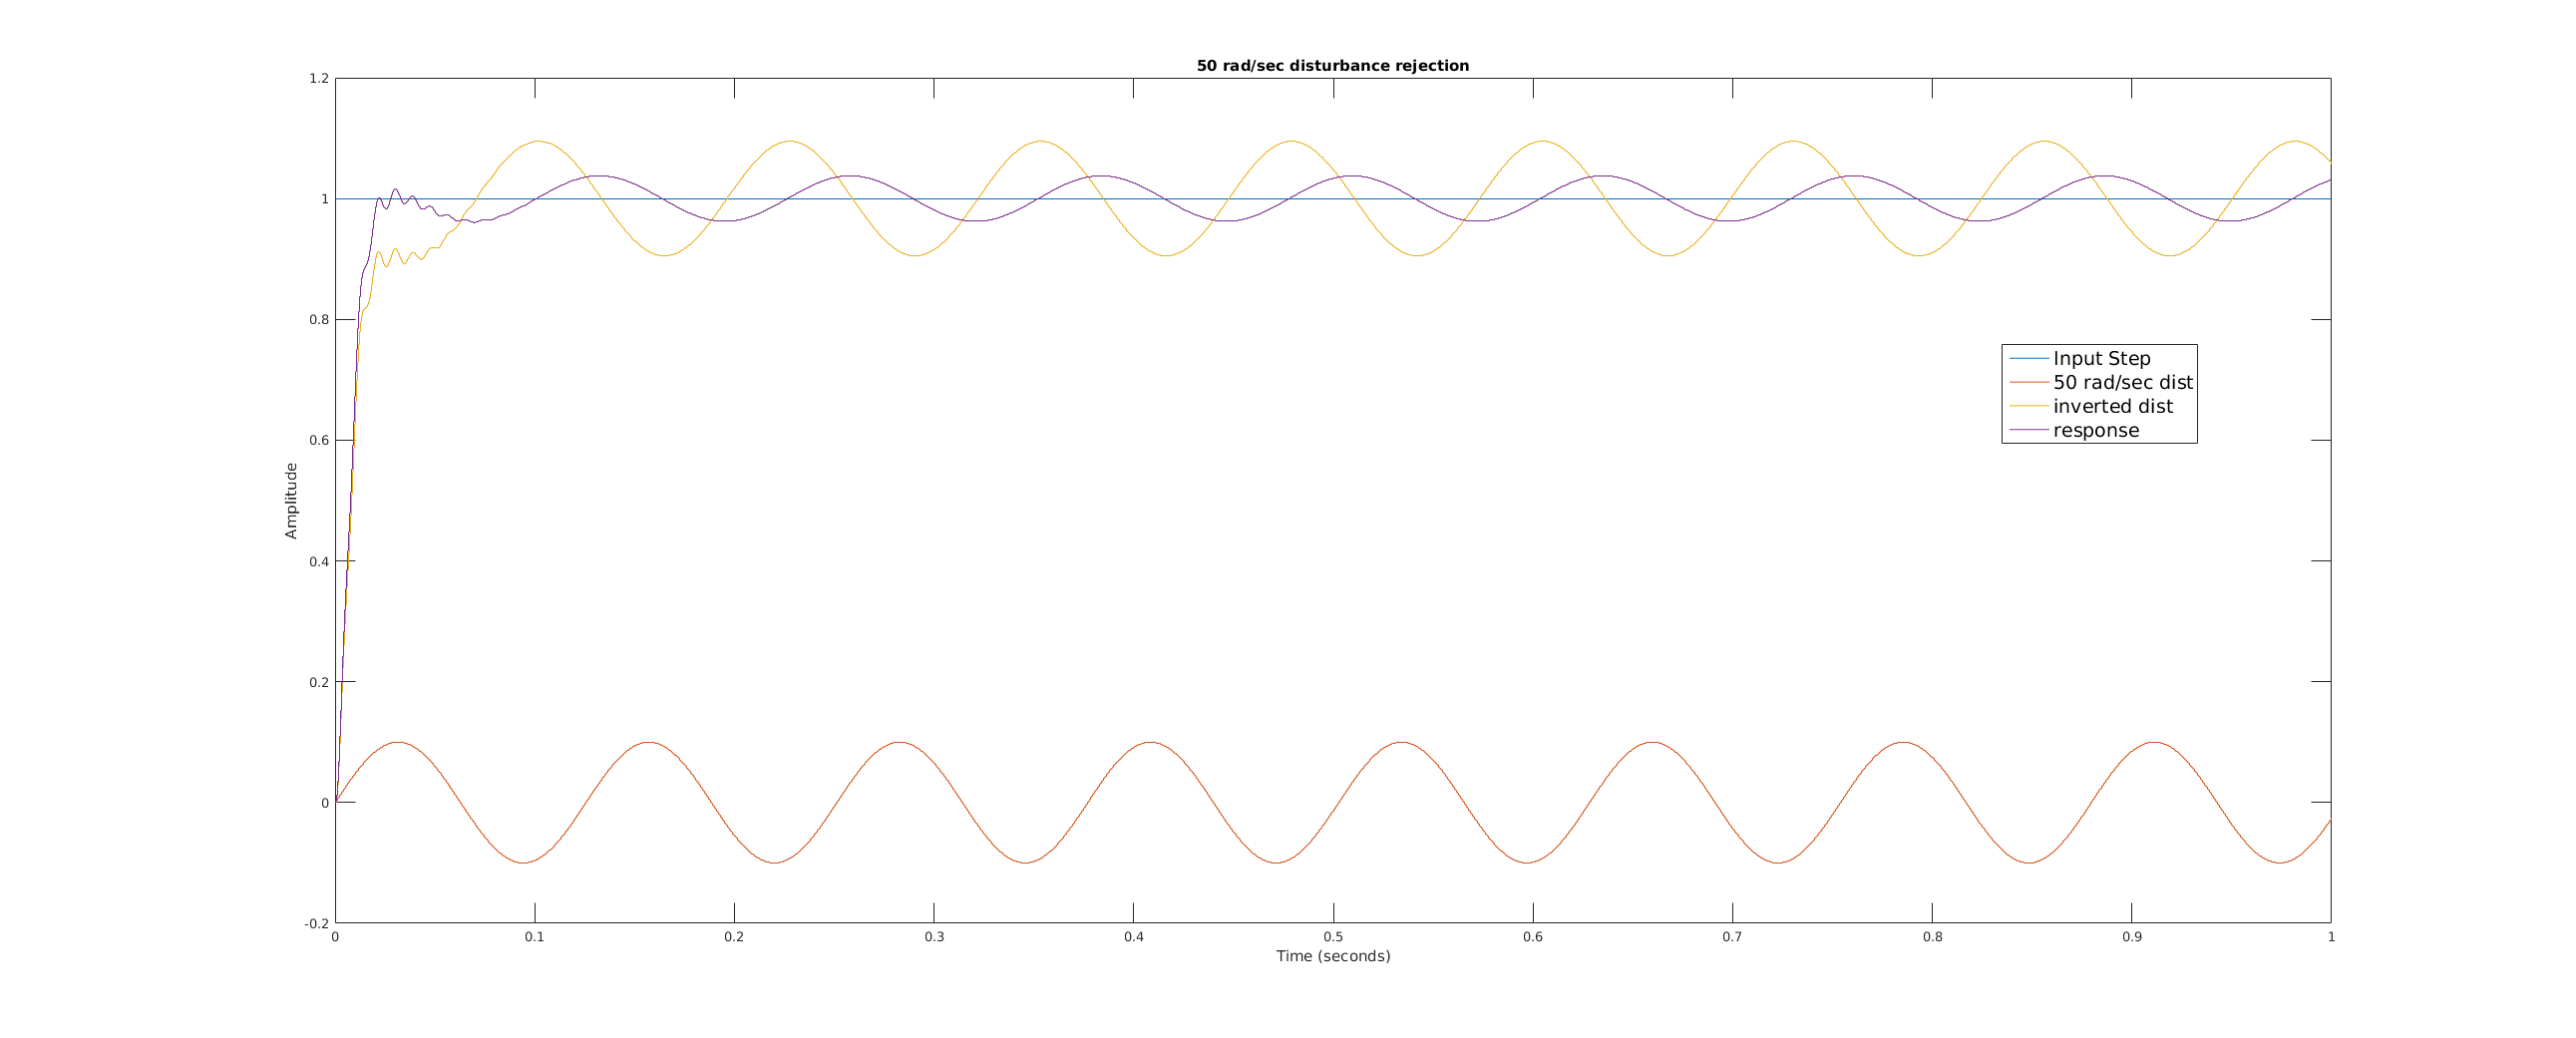
\includegraphics[width=0.9\textwidth]{Dist_50.png}
    \caption{The system response to an amplitude 1 step and a 50 rad/sec disturbance with amplitude 0.1.}
    \label{fig:Dist50radasec}
\end{figure}
Here, in Figure \ref{fig:Dist500radasec}, we see the feedforward control start to fail almost completely. The magnitude is now not high enough to cancel the disturbance and thus we see the full effect of the disturbance on the output.
\begin{figure}[H]
    \centering
    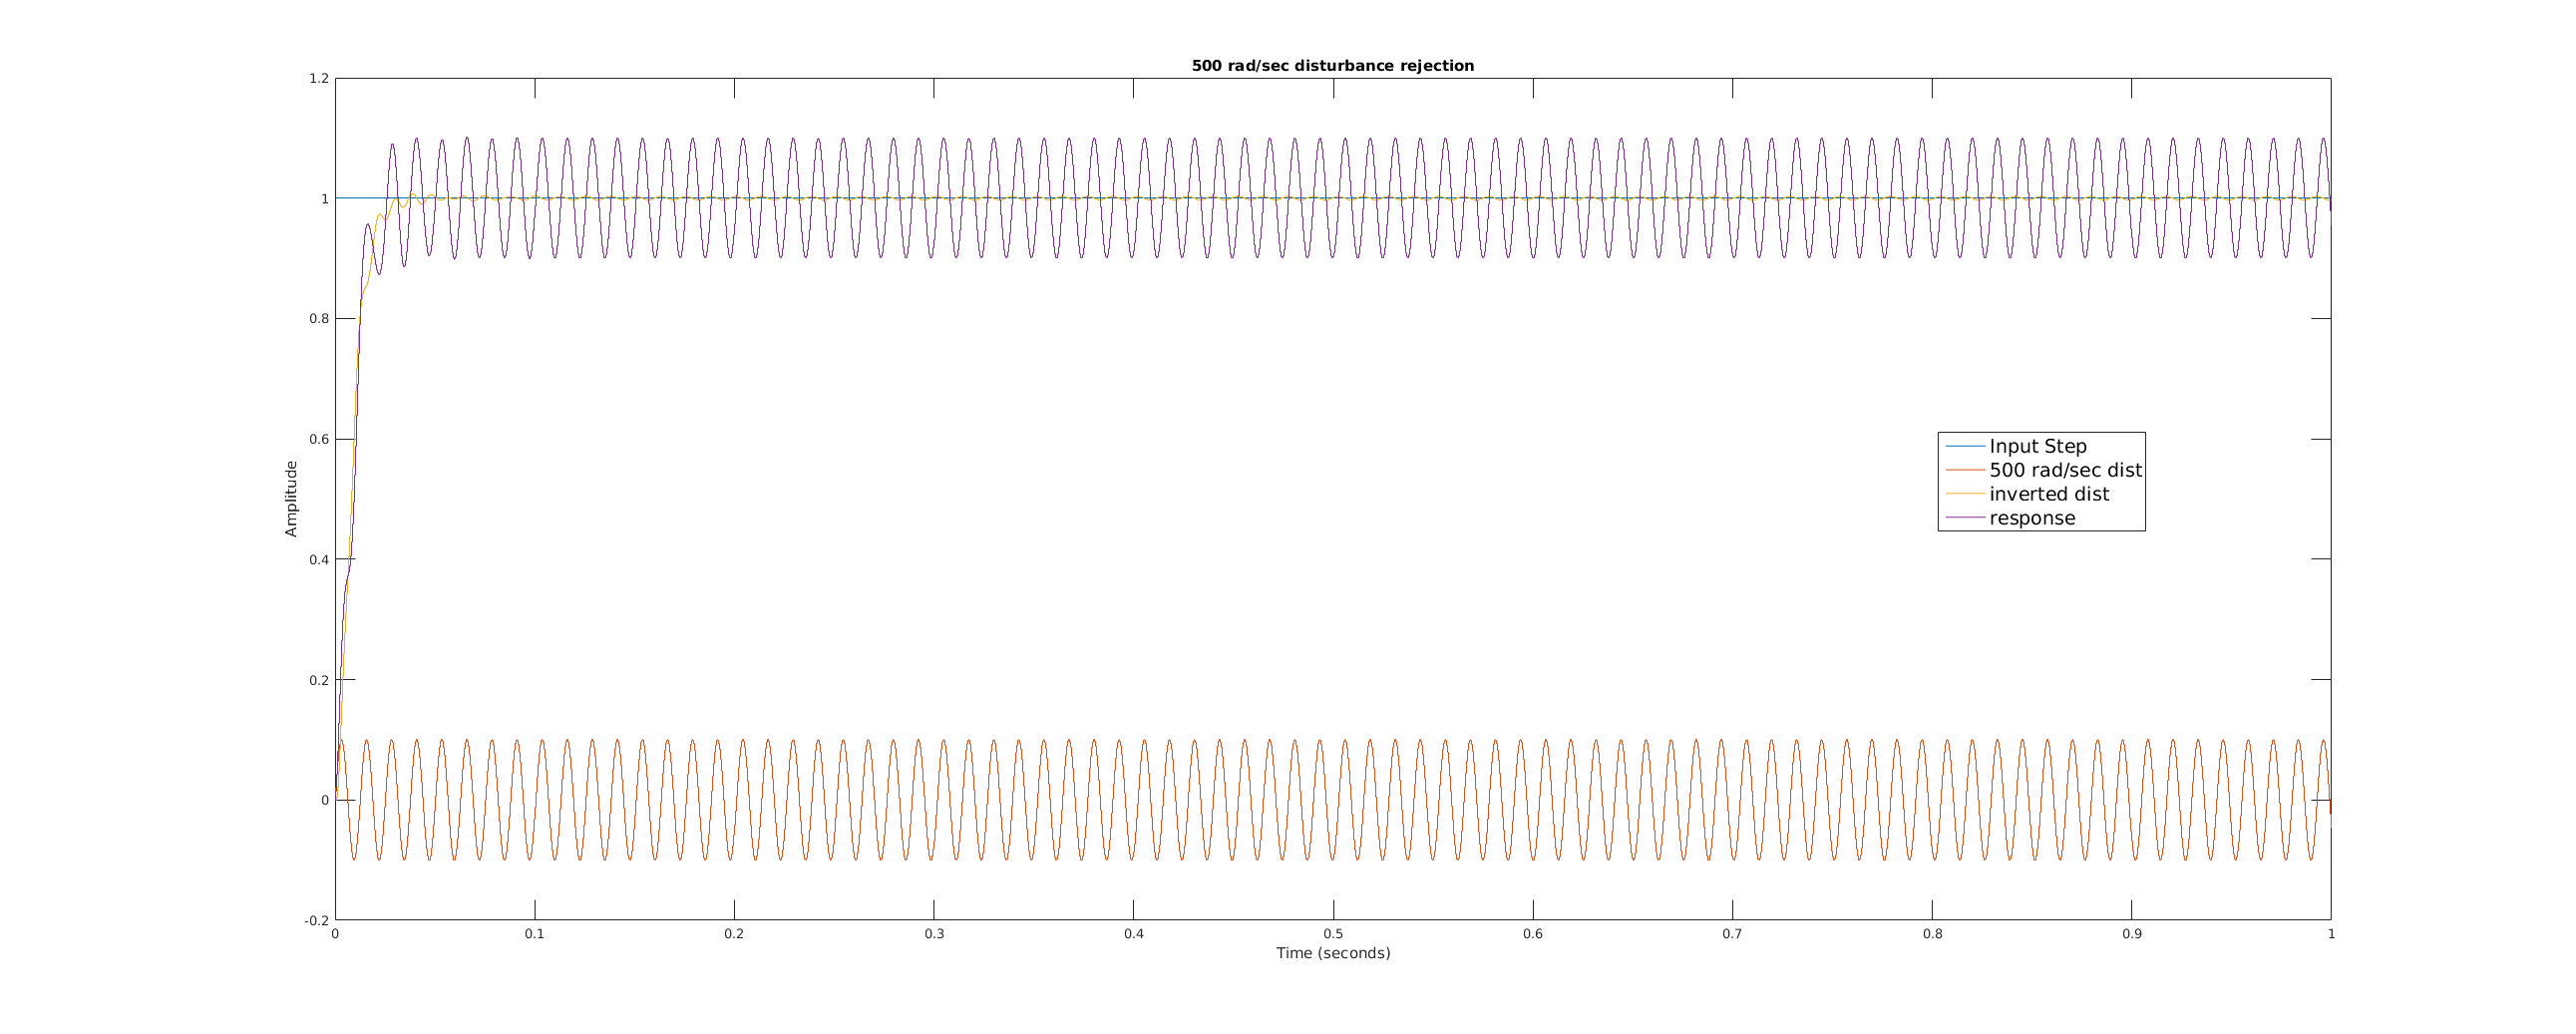
\includegraphics[width=0.9\textwidth]{Dist_500.png}
    \caption{The system response to an amplitude 1 step and a 500 rad/sec disturbance with amplitude 0.1.}
    \label{fig:Dist500radasec}
\end{figure}



\subsection{Simulation of State-Space Design}
Next, the state-space design results are shown. As mentioned in Section 2.3, Matlab's place function was used to determine $K$ and $L$.
\[ K = \left( \begin{array}{cccc}
1.765 & -1.2858 & 1.2585 & -0.8278
 \end{array} \right)\] 
 \[ L = \left( \begin{array}{c}
0.2419  \\
2.2437 \\
2.7681 \\
1.1430 \end{array} \right)\] 
In Figure \ref{fig:StepObs} we see the step response of our system with the observer and state feedback. The settling time is about 0.0025 seconds, which is just over a third of our goal. The rise time is also very low and we don't have much overshoot. This tells us we could probably push the settling time even further at the cost of overshoot.
\begin{figure}[H]
    \centering
    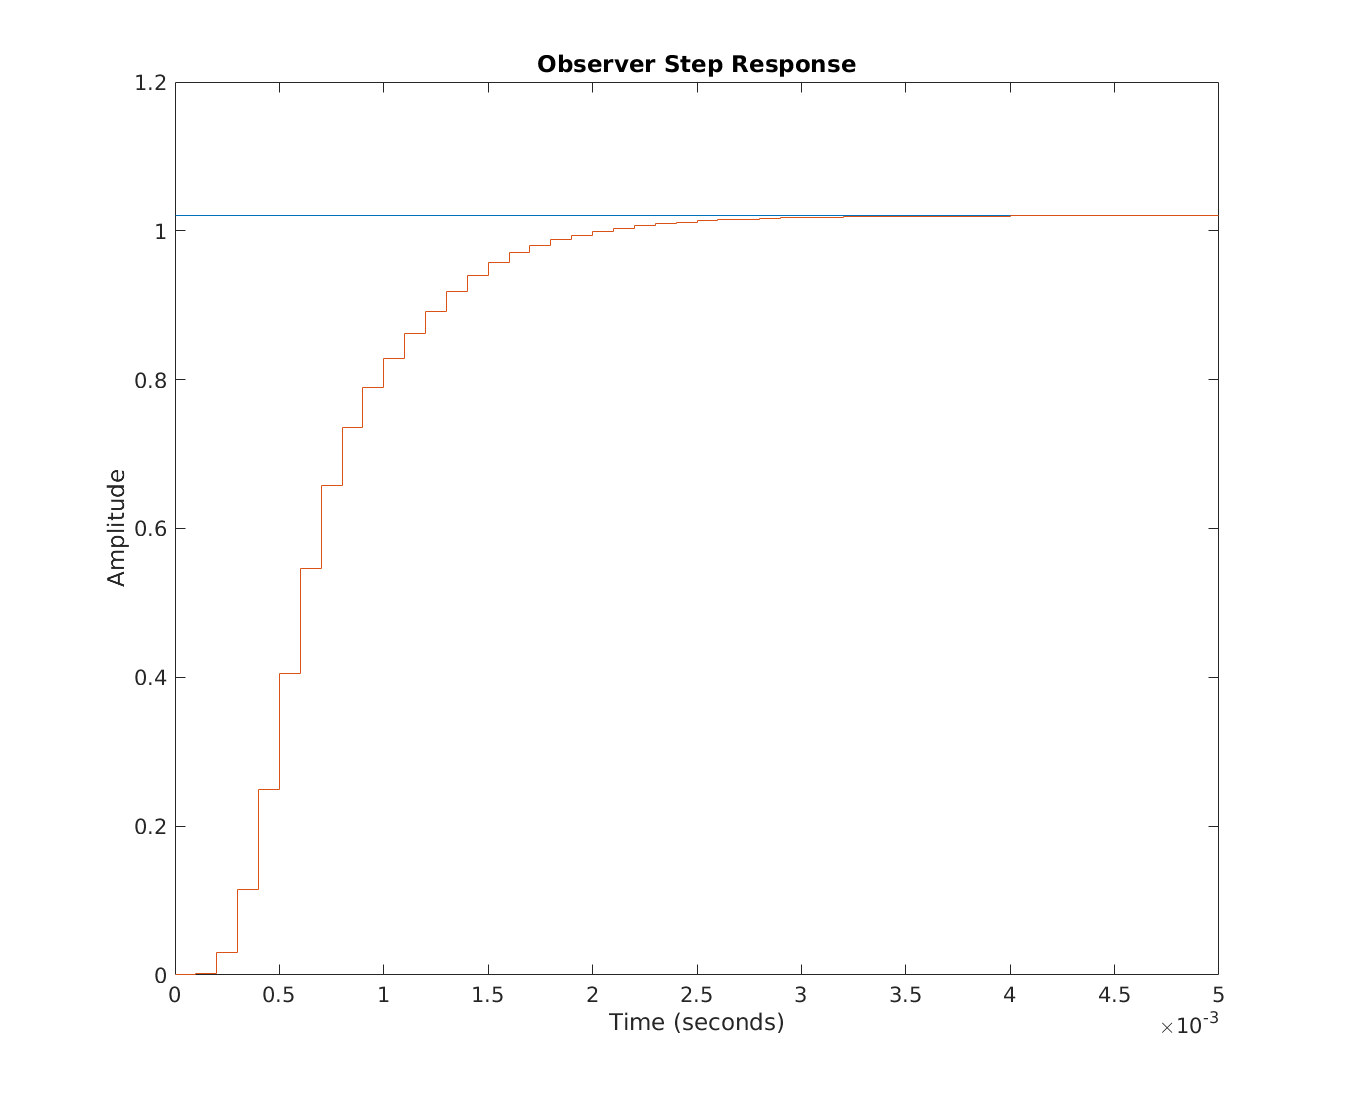
\includegraphics[width=0.8\textwidth]{OBSERVER_STEP.png}
    \caption{The step response of the system with an observer and state feedback. Note that the settling time is well within our goal of 0.007 seconds. Also note the lack of oscillations and general smooth response.}
    \label{fig:StepObs}
\end{figure}
Next we examine the pole and zero map of the total system to see if our poles ended up in the right spot. As is visible in Figure \ref{fig:Obspz} they aren't in quite the right place. We assume this is because place put the poles as close to our desired poles as possible. 
\begin{figure}[H]
    \centering
    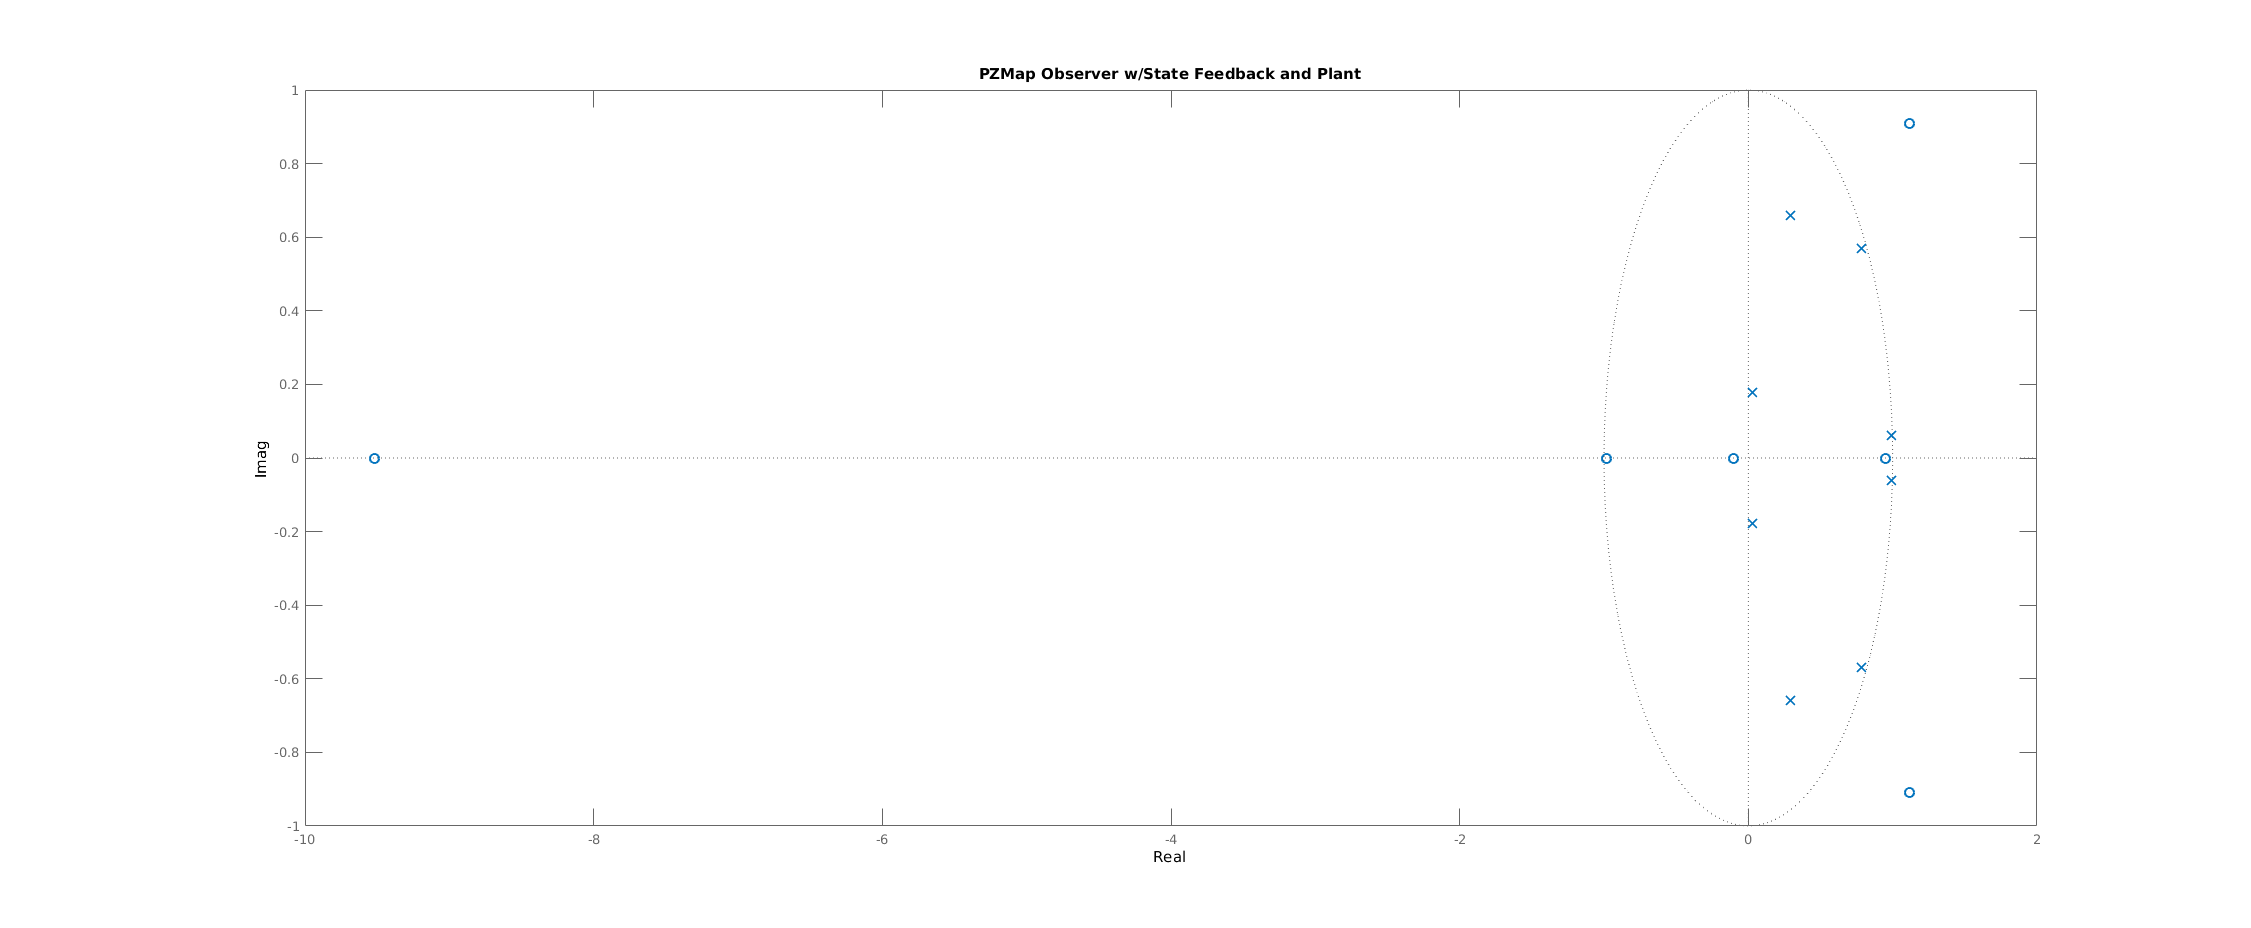
\includegraphics[width=\textwidth]{observer_pz.png}
    \caption{Pole Zero Map of the state space realization of $G(z)$ augmented with state feedback and an observer.}
    \label{fig:Obspz}
\end{figure}

\section{Discussion}
\subsection*{Errors in Design}
The main error I noticed in our design was that the pole placement didn't actually place the poles where we wanted. This can be seen in $\ref{fig:Obspz}$. I must assume this is due to the placement algorithm Matlab used or possibly the way we plotted the poles and zeros of the total system. This is also interesting because the response with the feedback observer has no overshoot, and that shouldn't be the case based on where the poles were placed. The design of our notch filters also wasn't
perfect, we would have like them to cancel the resonances better. This is difficult without going to higher-order filter models though.

\subsection*{Comparing PIF and State Feedback}
In comparing the PI with a two notch filters and the state feedback from a state estimator, it becomes clear the state feedback estimator is superior. The state estimator eliminates overshoot, and most importantly has a very fast settling time. It could have been further improved by introducing a matrix to adjust the reference's effect on the next state and another one to adjust the effect of the reference on the input. This would also have normalized the gain of our estimator and allowed us to
implement the feedforward controller with the state observer. Having said all that, the PI with notch filters doesn't perform badly. It does reduce the natural resonances of the system, just not to the extent the state feedback does. The settling time is also not quite as good either. It reaches a settling time of around 0.03 seconds, but can't get to the awesomeness of 0.003 seconds that the other one reaches. I would say that PI controllers are easy to use, they don't require
modification of the reference input and are much more common. There are also better tools for PID type controllers, allowing one to immediately see how the response of a system changes. They will probably also be less computationally intensive than all of the vector math in an estimator.

\subsection*{Feedforward Control}
The feedforward controller is awesome. The idea that we can measure a disturbance and then apply a control to reject it is sweet. Based on the bode diagram of the inverted plant, we kind of knew that higher frequencies would not be 180 degrees out of phase from the plant. This resulted in a partial cancellation of the disturbance, which can be seen in \ref{fig:Dist50radasec}. The magnitude term starts to fail at higher frequencies as well. It would be interesting to further explore a inverted plant that matched phase and magnitude better at these higher frequencies even if it effected the lower ones. Then one could measure the frequency of the disturbance and apply which ever inverted plant worked best. It would also be interesting to consider the case where the propagation of the disturbance from the measured location to the actuator head was not 1. That would result in our feedforward controller needing to implement the model of that propagation. Thus our feedforward controller would be $F(z)=\tilde{G}^{-1}(z)E(z)$. Overall, this was a very useful design even though it didn't work super well.



\section{Conclusion}
Together, Kaitlyn and I have implemented 2 different controllers to address our 4th order model of the tape drive system. We have explored state estimators and feedback, filtering resonant frequencies, and removing disturbances with an inverted plant model. The use of state estimators is extremely useful in monitoring of systems because one rarely has access to all of a systems states. Given that this estimation of states is accurate, which it should be if the estimator poles are fast enough
relative to the system poles, one can use state feedback to give inputs into a system that move the poles to a desired location.
Thus, modifying the characteristics of a system. I could then use this same concept to build an estimator of disturbances, and even calculate the optimal input to change a systems states from one point to another based on the estimated states.

Filtering is also an essential tool in control design that we have applied here. Being able to reduce resonances in a system can help it maintain stability and it is always nice to come back and use this. The feedforward design we made is also great experience. The core idea behind this was inverting the plant model, which is always a difficult task when unstable zeros exist. In general inverting the plant model is the goal of all controllers because it means the output should be equivalent
to the reference. This was also useful because we got experience with disturbance rejection. In this case we were modeling a measure of the disturbance beforehand, but the same concept can be applied to data coming in after the initial disturbance.

In the future it would be interesting to explore several other features of this system. For one, we could try to build a better model for the inversion of the plant. This would hopefully allow us to reject disturbances better. Also, we could explore changing sample rates to see how that effected the stability and response. After that, it would be nice to build a state estimator that modeled the disturbance and dealt with the reference input properly. Finally, we could use a quadratic
regulator or Kalman Filter to find the optimal control inputs to the system.

Overall, this was a very useful project exploring an interesting plant system with multiple techniques. It broadened our knowledge of discrete domain design, especially with reference to rejection of measured disturbances and state estimation. I personally appreciated it and would like to work more on control problems like this.

\clearpage
\appendix
\section*{Code Appendix}
\lstinputlisting{prog1.m}

\begin{thebibliography}{10} 
	\bibitem{thesis} Zhong, Hua."Advanced Controller Designs for Head Positioning and Tension Regulation in Tape Drive Systems." Ph.D Thesis, 2014.
	\bibitem{notchF} S. C. D. Roy, B. Kumar, and S. B. Jain,"FIR notch filter design - A Review", Facta Univ. (Niscaron,), Ser. Electron. Energetics, vol. 14, no. 3, pp. 295-327, 2001.
\end{thebibliography}
\end{document}
